\documentclass[6008notes.tex]{subfiles}
\begin{document}
\graphicspath{ {images/indepstruct/} }

\section{Independence Structure}

\subsection{Independent Events}

When you flip a coin or roll dice, the outcome of a coin flip or a die roll isn't going to tell you anything about the outcome of a new coin toss or die roll unless you have some very peculiar coins or dice.

we're going to formalize this by saying that two events A and B are independent, which we'll denote by this thing that looks like an upside down T: $\bigCI$

{\centering $A \bigCI B \qquad \text{if} \qquad \mathbb {P}(A \cap B) = \mathbb {P}(A) \mathbb {P}(B)$ \par}

If $\mathbb {P}(A) > 0$ we can use the product rule for events to rewrite the left side:

{\centering $\mathbb {P}(B \mid A) \mathbb {P}(A) = \mathbb {P}(A) \mathbb {P}(B)$ \par}

Cancelling $\mathbb {P}(A)$ on both sides:

{\centering $A \bigCI B \qquad \text{if} \qquad \mathbb {P}(B \mid A) = \mathbb {P}(B)$ \par}

Similarly, if $\mathbb {P}(B) > 0$

{\centering $A \bigCI B \qquad \text{if} \qquad \mathbb {P}(A \mid B) = \mathbb {P}(A)$ \par}

So knowing $B$ doesn't tell us anything new about $A$, and \textit{vice versa}.

\subsection{Independent Random Variables}

$X$ and $Y$ are independent ($X \bigCI Y$) if $p_{X,Y} (x,y) = p_X(x)p_Y(y)$.

Knowing one gives no information about the other, so $p_{X \mid Y} (x \mid y) = p_X(x)$.

\paragraph{Exercise: Independent Random Variables}  In this exercise, we look at how to check if two random variables are independent in Python. Please make sure that you can follow the math for what's going on and be able to do this by hand as well.

Consider random variables $W$, $I$, $X$, and $Y$, where we have shown the joint probability tables $p_{W,I}$ and $p_{X,Y}$.

{\centering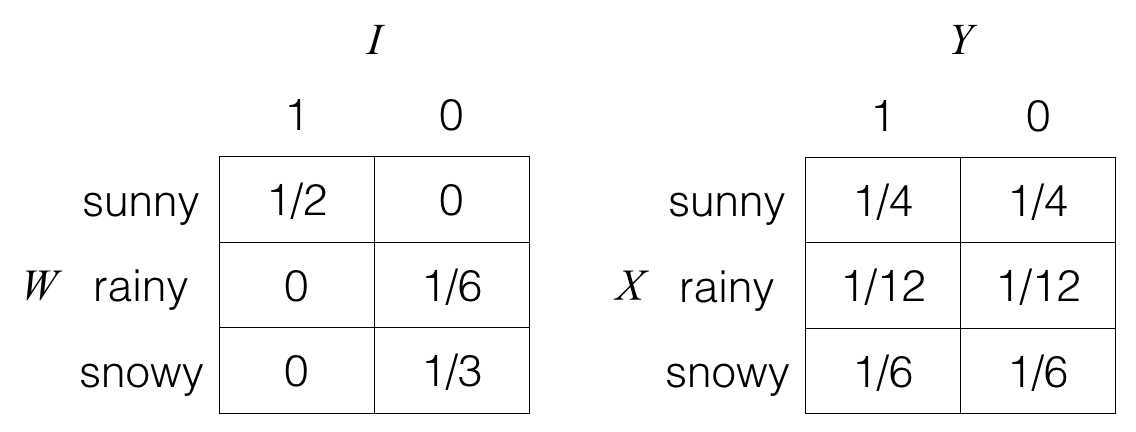
\includegraphics[scale=0.4]{images_sec-joint-rv-ex-marg} \par}

In Python:

\begin{lstlisting}
prob_W_I = np.array([[1/2, 0], [0, 1/6], [0, 1/3]])
\end{lstlisting}

Note that here, we are not explicitly storing the labels, but we'll keep track of them in our heads. The labels for the rows (in order of row index): sunny, rainy, snowy. The labels for the columns (in order of column index): 1, 0.

We can get the marginal distributions $p_W$ and $p_I$:

\begin{lstlisting}
prob_W = prob_W_I.sum(axis=1)
prob_I = prob_W_I.sum(axis=0)
\end{lstlisting}

Then if $W$ and $I$ were actually independent, then just from their marginal distributions $p_W$ and $p_I$, we would be able to compute the joint distribution with the formula:

{\centering$\text {If $W$ and $I$ are independent:} \qquad p_{W,I}(w,i)=p_ W(w)p_ I(i) \qquad \text {for all }w,i.$ \par}
 
Note that variables \lstinline{prob_W} and \lstinline{prob_I} at this point store the probability tables $p_W$ and $p_I$ as 1D NumPy arrays, for which NumPy does \textit{not} store whether each of these should be represented as a row or as a column.

We could however ask NumPy to treat them as column vectors, and in particular, taking the outer product of \lstinline{prob_W} and \lstinline{prob_I} yields what the joint distribution would be if $W$ and $I$ were independent:

\begin{eqnarray*}
\begin{bmatrix}
p_W(\text{sunny}) \\
p_W(\text{rainy}) \\
p_W(\text{snowy})
\end{bmatrix}
\begin{bmatrix}
p_I(1) & p_I(0)
\end{bmatrix}
=
\begin{bmatrix}
p_W(\text{sunny})p_I(1) & p_W(\text{sunny})p_I(0) \\
p_W(\text{rainy})p_I(1) & p_W(\text{rainy})p_I(0) \\
p_W(\text{snowy})p_I(1) & p_W(\text{snowy})p_I(0)
\end{bmatrix}.
\end{eqnarray*}

The left-hand side is an outer product, and the right-hand side is precisely the joint probability table that would result if $W$ and $I$ were independent.

To compute and print the right-hand side, we do:

\begin{lstlisting}
print(np.outer(prob_W, prob_I))
\end{lstlisting}


\subsection{Mutual vs Pairwise Independence}

To extend the independence story to more than two variables, the strongest way is by using something called ``mutual independence''. We'll say that three random variables  $X$, $Y$, and $Z$ are mutually independent if we can write  the joint distribution as simply the product of the three individual distributions:

{\centering$p_{X,Y,Z} (x,y,z) = p_X(x) p_Y(y) p_Z(z)$ \par}

Knowing $X$ and $Y$ won't tell you anything about $Z$. Knowing $X$ won't tell you anything about $Y$. They're completely independent.

There are also weaker forms of independence that we're interested in, for example, ``pairwise independence''. This means that for any two variables, you can write:

{\centering$p_{X,Y} (x,y) = p_X(x) p_Y(y)$ \par}

and similarly for $Y,Z$ and $X,Z$. This is saying if I know any one, it doesn't tell me think anything about any of the others. But this is not the same as mutual independence, it's not as strong.

As an example of why, suppose that we have two random variables $X$ and $Y$. They both represent independent fair coin flips. We'll write the outcomes as 0 and 1, and each one has a 50-50 chance of being heads or tails, 0 or 1.

We'll define $Z = X \oplus Y$, where ``XOR'' (written $\oplus$) is defined to be a function that takes in two things and returns 1 when exactly one of them is 1:

\begin{center}
\begin{tabular}{| c | c | c }
\textbf{x} & \textbf{y} & \textbf{z} \\
\hline
0 &	0 &	0 \\
0 &	1 &	1 \\
1 &	0 &	1 \\
1 &	1 &	0 \\
\end{tabular}
\end{center}

What's the probability $p_{X,Y}$ for each of these configurations? They're independent fair coin flips, so each is equally likely. The probability of any particular one is 0.5 for $X$ times 0.5 for $Y$, so 0.25:

\begin{center}
\begin{tabular}{| c | c | c | c }
$\mathbf{p_{X,Y}}$ & \textbf{x} & \textbf{y} & \textbf{z} \\
\hline
0.25 & 0 &	0 &	0 \\
0.25 & 0 &	1 &	1 \\
0.25 & 1 &	0 &	1 \\
0.25 & 1 &	1 &	0 \\
\end{tabular}
\end{center}

What's the distribution for Z? There are two ways to get $z=0$ and they each have probability 0.25. If we add them up then we have a 0.5 chance of $z$ being 0 and similarly a 0.5 chance of $z$ being 1. 

\begin{eqnarray*}
p_Z(z)
&=&
\begin{cases}
  0.5 & \text{if }z=0 \\
  0.5 & \text{if }z=1
\end{cases}
\end{eqnarray*}

What's $Z$ given $X$? Well, it's actually the same. If $x=0$, then we can restrict ourselves to just looking at the top two rows of the table, so Z can either be 0 or 1. And, again, they're equally likely so it's 50-50. If $x=1$, we can just look at the bottom two rows, and again they're equally likely, 50-50. 

\begin{eqnarray*}
p_{Z \mid X}(z \mid x)
&=&
\begin{cases}
  0.5 & \text{if }z=0 \\
  0.5 & \text{if }z=1
\end{cases}
\end{eqnarray*}

So $p_{Z \mid X}(z \mid x) = p_Z(z)$, it doesn't depend on X at all. So this means that $Z \bigCI X$.

By symmetry, we can make the same argument for $Z \bigCI Y$, and we said at the start that $X \bigCI Y$. So here we have three random variables that are all pairwise independent --- if you look at any pair, knowing one doesn't tell you about the other. 

But if we look all together, they're not mutually independent. For example, if I know any two of them, then I know exactly what the third one is going to be. The distribution over the third one changes from being fair 50-50 to being deterministic. For example, if $X$ is 0 and $Y$ is 0, then $Z$ is also going to be 0. And if I didn't know that, then the probability would be 50-50. Once I do know that, the probability becomes 1 that it's 0 and 0 that it's anything else. So here, they're not mutually independent. In this example it may seem a little contrived, but in general, it's often tempting to assume that knowing things are pairwise independent tells you that they're mutually independent. But you have to be aware that they're not.

\subsection{Conditional Independence}

We say that two random variables $X$ and $Y$ are conditionally independent given the third random variable $Z$ if we can write the conditional distribution for both of them as the product of the individual conditionals:

{\centering$p_{X,Y \mid Z} (x,y \mid z) = p_{X \mid Z} (x \mid z) p_{Y \mid Z} (y \mid z) $ \par}

Intuitively, this means that once we know $Z$, then knowing something about $Y$ doesn't tell you anything about $X$, and \textit{vice versa}. 

Notice that marginal independence and conditional independence are not the same thing. So if you have marginal independence, then that does not necessarily imply conditional independence. And the reverse is also not true. So two random variables $X$ and $Y$ could be independent but not conditionally independent given something else. Or two random variables could be conditionally independent but not marginally independent given something else. 

As an example that illustrates this, suppose we have three random variables $R$, $S$, and $T$. We'll ask two questions: $(a)$ is $S \bigCI T$? $(b)$ is $S \bigCI T \mid R$? There are two different ways of writing the joint distribution:

\begin{eqnarray*}
(a) p_{R,S,T}(r,s,t) &=& p_R(r) p_{S \mid R}(s \mid r)  p_{T \mid R}(t \mid r) \\
(b) p_{R,S,T}(r,s,t) &=& p_S(s) p_T(t) p_{R \mid S,T}(r \mid s,t) 
\end{eqnarray*}

%If we were to draw a little diagram for R, S, and T, then we would say first is R. Then from R, there's S. So R kind of tells you how to get S. And then from R, there's T. So once we have this, now we can answer our questions we posed before. Is S independent of T, and is S independent of T given R? So we'll 

\paragraph{Part $(a)$:} To determine whether two things are independent we just write out the distribution and see if it factors --- that is, see if we can write it as something that only depends on $S$ times something that only depends on $T$. If we can, then the former is $p_S(s)$, the latter is $p_T(t)$. 

To compute the distribution of $p_{S,T}(s,t)$ from $p_{R,S,T}(r,s,t)$, we just have to sum over every possible value of $r$:

\begin{eqnarray*}
p_{S,T}(s,t) &=& \sum_r p_{R,S,T}(r,s,t) \\
             &=& \sum_r p_R(r) p_{S \mid R}(s \mid r)  p_{T \mid R}(t \mid r) \\
						 &\neq& p_S(s) p_T(t)
\end{eqnarray*}

In general, we will not be able to factor the result because it will be a sum of different things that depend on $S$ and $T$ in different ways. So therefore, $S$ and $T$ are not independent. 

Are they conditionally independent given $R$? To compute that, we have to see whether $p_{S,T}(s,t) \mid R = p_{S \mid R}(s \mid r)  p_{T \mid R}(t \mid r)$. To compute a conditional distribution, remember that we just have to divide by the distribution of whatever we're conditioning on:

\begin{eqnarray*}
p_{S,T \mid R}(s,t \mid r) &=& \frac{p_{R,S,T}(r,s,t)}{p_R(r)} \\
             &=& \frac{p_R(r) p_{S \mid R}(s \mid r)  p_{T \mid R}(t \mid r)}{p_R(r)} \\
						 &=& p_{S \mid R}(s \mid r)  p_{T \mid R}(t \mid r)
\end{eqnarray*}

Canceling $p_R(r)$ leaves us with exactly the two terms we want. So the joint conditional distribution  becomes the product of the two individual conditionals. So $S$ and $T$ are, in fact, conditionally independent given $R$.

\paragraph{Part $(b)$:}  We have that 

{\centering$p_{R,S,T}(r,s,t) = p_S(s) p_T(t) p_{R \mid S,T}(r \mid s,t)$ \par}

%p R S T is p S times p T times p R given S T. So if we were to draw our little diagram for this one, it would be-- well, we start with S. Then we start with T. So we start with S and T. And from there, we get R given both of them. So given both of them, we have R. And we're interested in the two questions, is S independent of T and is S independent of T given R? So let's look at the first question. 

As in part $(a)$, if we want to compute whether $S$ and $T$ are independent, we have to look at the joint distribution and see whether we can write it as a product of the two individual distributions. 

Again, to compute the joint distribution we have sum over every possible $r$:

\begin{eqnarray*}
p_{S,T}(s,t) &=& \sum_r p_S(s) p_T(t) p_{R \mid S,T}(r \mid s,t) \\
             &=& p_S(s) p_T(t) \sum_r p_{R \mid S,T}(r \mid s,t) \\
						 &=& p_S(s) p_T(t)
\end{eqnarray*}

As $p_S(s)$ and $p_T(t)$ don't depend on $r$ they can be factored outside the summation. But no matter what $S$ and $T$ are, if we sum over every possible value of $r$, then $\sum_r p_{R \mid S,T}(r \mid s,t)$ is just going to give us 1 because it is just a probability distribution over R, and all probability distributions have to sum to 1. Hence $p_{S,T}(s,t) = p_S(s) p_T(t)$, and that's exactly the condition for independence. So in this case, $S \bigCI T$. 

What about conditional independence? As in part $(a)$, we have to look at the conditional distribution $p_{S,T \mid R}(s,t \mid r)$ and see whether it factors.

{\centering$p_{S,T \mid R}(s,t \mid r) = \frac{p_S(s) p_T(t) p_{R \mid S,T}(r \mid s,t)}{p_R(r)}$ \par}

If we try to factor this, we'll see that we run into trouble when we get to the term $p_{R \mid S,T}(r \mid s,t){p_R(r)}$ because in general, this is not going to factor. We don't know how S and T interact here, and there are no simplifications we can do to make this term go away. So here, $S \nbigCI T \mid R$. 

We've seen from the last two examples that sometimes we can have marginal independence without conditional independence, and that sometimes we can have conditional independence without marginal independence. So it's important to keep in mind that these two are not always the same thing, and knowing one doesn't necessarily tell you the other.

\subsection{Explaining Away}

Let's look at an example with conditional probability. Suppose we have three events, $R$, $A$, and $T$, where
\begin{itemize}
\item $R$ is the event that a Red Sox game 
\item $A$ is the event there's an accident downtown
\item $T$ is the event there is unusually bad traffic
\end{itemize}

The chance of having a game and the chance of having an accident are each independently 50:50 : 

\begin{eqnarray*}
p_R(r)
&=&
\begin{cases}
0.5 & r=1\\
0.5 & r=0.
\end{cases} \\
p_A(a)
&=&
\begin{cases}
0.5 & a=1\\
0.5 & a=0.
\end{cases}
\end{eqnarray*}

Whether or not there is traffic depends on whether there's a game and whether there's an accident. This table shows the probability that $T$ is 1 for each configuration of $r$ and $a$:

\begin{center}
\begin{tabular}{ c  c | c }
\textbf{r} & \textbf{a} & $p_{T \mid R,A} (1 \mid r,a)$ \\
\hline
0 &	0 &	0.3 \\
0 &	1 &	0.9 \\
1 &	0 &	0.9 \\
1 &	1 &	0.3 \\
\end{tabular}
\end{center}

So with no game and no accident, the probability of having bad traffic is 0.3. With either or both, then the probability goes up to 0.9. The table shows us the distribution for $T = 1$. The distribution for $T = 0$ would just have 1 minus this in every entry. 

We want to calculate three probabilities:\\
(a) $\mathbb{P}(R = 1)$ \\
(b) $\mathbb{P}(R = 1 \mid T = 1)$ \\
(b) $\mathbb{P}(R = 1 \mid T = 1, A = 1)$ 

Part (a) is easy, as $\mathbb{P}(R = 1)$ is given to us as 0.5. But in (b) and (c), we're asked to find information about $R$ given $T$, whereas the problem setup gives us information about $T$ in terms of $R$. So we'll use Bayes' rule to turn the conditioning around. In both cases, we're only interested in the case where $T = 1$, so we'll not worry about the full distribution for now.

Bayes' rule tells us that 

{\centering$p_{R,A \mid T}(r,a \mid 1) = \frac{p_{T \mid R,A}(1 \mid r,a) p_R(r) p_A(a)}{p_T(1)}$ \par}

%this is the probability of p T given R A times p of R and A, which is since they're independent just a product of the two, and divided by p T. Sorry, this should be a 1. Because we're only interest in the case where T is 1.   So we're interested in this thing for different values of R and A. And since this is going to be a distribution over R and A, anything that we get is going to have to sum up to 1 for every possible value, that is the four different possibilities for R and A should all sum up, the probabilities should all sum up to 1. And 

If we look carefully, we'll see that, in this case, because $R$ and $A$ are independent 50-50, $p_R(r)$ and $p_A(a)$ are going to be the same for every combination of $r$ and $a$. Similarly, the denominator is also going to be the same for every $r$ and $a$. So we can take a shortcut and say that these terms together are equal to some constant $C$:

{\centering$p_{R,A \mid T}(r,a \mid 1) = C \cdot p_{T \mid R,A}(1 \mid r,a)$ \par}

The table for $p_{T \mid R,A}(1 \mid r,a)$ is shown above, and we know that $p_{R,A \mid T}(r,a \mid 1)$ is some constant times this table. The probabilities are 0.3, 0.9, 0.9, 0.9. Except we know that they have to sum to 1. So if we take everything and divide by their sum, we get the normalized distribution of $r$ and $a$ given $t=1$. 

\begin{center}
\begin{tabular}{c c | c  c}
 & & \textbf{a} & \\
 & & 0 & 1 \\
\hline
\textbf{r} & 0 &	0.1 &	0.3 \\
 & 1 &	0.3 &	0.3 \\
\end{tabular}
\end{center}

In part (b), we're asking for $\mathbb{P}(R = 1 \mid T = 1)$. So in this case, we don't care about $a$, we only care about $r$ being 1 and we're marginalizing over A. So from the bottom row of the normalized distribution,  $\mathbb{P}(R = 1 \mid T = 1) = 0.3 + 0.3 = 0.6$.

In part (b), we're asking for $\mathbb{P}(R = 1 \mid T = 1, A = 1)$. If we condition on $a=1$, then we're restricting ourselves to the right column:

\begin{center}
\begin{tabular}{c c | c}
 & & \textbf{a} \\
 & & 1 \\
\hline
\textbf{r} & 0 &	0.3 \\
           & 1 &	0.3 \\
\end{tabular}
\end{center}

The probability that $r = 1$ is 0.3 divided by the marginal probability of the column, that is 0.3 divided by 0.6. It occurs half the time because it's equally likely to be 0 or 1. So here our probability goes back down to 0.5. Intuitively, why is this? Why does our probability change? When we had more information the first time, in (b), $T = 1$, our probability went up from 0.5 to 0.6. But when we added even more information, then it went back down. 

If we go back and look at the scenario, what this is asking is only given that there is traffic, what's the probability that there was a game? Well, it's a little higher in (b) because we know games cause traffic. So if there was traffic, then it's reasonable to assume that there was a game. So the probability goes up. But we know that both games and accidents cause traffic. So if we know that there was traffic and we know there was an accident, in (c), then it's more likely that the traffic was caused by the accident. So this is called explaining away, where once we observe one explanation, that is the accident, our belief in a different explanation, the Red Sox game, goes back down.  

\subsection{Practice Problem: Conditional Independence}

Suppose $X_0, \dots , X_{100}$ are random variables whose joint distribution has the following factorization:

{\centering$p_{X_0, \dots , X_{100}}(x_0, \dots , x_{100}) = p_{X_0}(x_0) \cdot \prod _{i=1}^{100} p_{X_ i | X_{i-1}}(x_ i | x_{i-1})$ \par}
 
This factorization is what's called a Markov chain. We'll be seeing Markov chains a lot more later on in the course.

Show that $X_{50} \perp X_{52} | X_{51}$.

Solution: Notice that we can marginalize out $x_{100}$ as such:

{\centering$p_{X_0, \dots , X_{99}}(x_0, \dots , x_{99}) = p_{X_0}(x_0) \cdot \prod _{i=1}^{99} p_{X_ i | X_{i-1}}(x_ i | x_{i-1}) \cdot \underbrace{\sum _{x_{100}} p_{X_{100}|X_{99}}(x_{100}|x_{99})}_{= 1} \qquad\qquad$ (2.5) \par}
 
Now we can repeat the same marginalization procedure to get:

{\centering$p_{X_0, \dots , X_{50}}(x_0, \dots , x_{50}) = p_{X_0}(x_0) \cdot \prod _{i=1}^{50} p_{X_ i | X_{i-1}}(x_ i | x_{i-1})$ \par}

In essence, we have shown that the given joint distribution factorization applies not just to the last random variable ($X_{100}$), but also up to any point in the chain.

For brevity, we will now use $p(x_{i}^{j})$ as a shorthand for $p_{X_ i, \dots , X_{j}}(x_ i, \dots , x_{j})$. We want to exploit what we have shown to rewrite $p(x_{50}^{52})$

\begin{eqnarray*}
		p(x_{50}^{52})
        &=& \sum_{x_{0} \dots x_{49}} \sum_{x_{53} \dots x_{100}} p(x_{0}^{100}) \\
		&=& \sum_{x_{0} \dots x_{49}} \sum_{x_{53} \dots x_{100}} \left[p(x_{0}) \prod_{i=0}^{50} p(x_{i}|x_{i-1})\right] \cdot p(x_{51}|x_{50}) \cdot p(x_{52}|x_{51}) \cdot \prod_{i=53}^{100} p(x_{i}|x_{i-1}) \\
		&=& \sum_{x_{0} \dots x_{49}} \sum_{x_{53} \dots x_{100}} p(x_{0}^{50}) \cdot p(x_{51}|x_{50}) \cdot p(x_{52}|x_{51}) \cdot \prod_{i=53}^{100} p(x_{i}|x_{i-1}) \\
		&=& p(x_{51}|x_{50}) \cdot p(x_{52}|x_{51}) \cdot \sum_{x_{0} \dots x_{49}} p(x_{0}^{50}) \underbrace{\sum_{x_{53} \dots x_{100}} \prod_{i=53}^{100} p(x_{i}|x_{i-1})}_{=1} \\
		&=& p(x_{51}|x_{50}) \cdot p(x_{52}|x_{51}) \cdot \sum_{x_{0} \dots x_{49}} p(x_{0}^{50}) \\
		&=& p(x_{50}) \cdot p(x_{51}|x_{50}) \cdot p(x_{52}|x_{51})
    \end{eqnarray*}
		
where we used (2.5) for the 3rd equality and the same marginalization trick for the 5th equality. We have just shown the Markov chain property, so the conditional independence property must be satisfied.

\end{document}